\documentclass[conference]{IEEEtran}
\IEEEoverridecommandlockouts
\usepackage{cite}
\usepackage{amsmath,amssymb,amsfonts}
\usepackage{algorithmic}
\usepackage{graphicx}
\usepackage{textcomp}
\usepackage{xcolor}
\usepackage{booktabs}
\usepackage{multirow}
\usepackage{array}
\usepackage{url}
\usepackage{float}
\usepackage{makecell}
\setlength{\textfloatsep}{8pt plus 2pt minus 4pt}
\setlength{\floatsep}{8pt plus 2pt minus 4pt}
\setlength{\intextsep}{8pt plus 2pt minus 4pt}
\def\BibTeX{{\rm B\kern-.05em{\sc i\kern-.025em b}\kern-.08em
    T\kern-.1667em\lower.7ex\hbox{E}\kern-.125emX}}
\begin{document}

\title{Towards Accurate Multi-Class Ocular Disease Classification: An Explainable Ensemble Deep Learning Approach with Grad-CAM}

\author{}

\maketitle
\vspace{-3em}

\begin{abstract}
Timely and accurate detection of ocular diseases is essential for preventing irreversible vision loss. However, access to trained ophthalmologists remains limited in many parts of the world. Existing deep learning studies mainly focus on single-disease classification, evaluate only a few models, and often lack explainability. These limitations reduce their practical use in clinical settings. In order to overcome the above-mentioned shortcomings, an explainable deep learning framework for multi-class classification of fundus images in the categories of cataract, diabetic retinopathy, glaucoma, and normal classes is proposed. The framework consists of morphological cropping, pixel normalization, CLAHE enhancement and data augmentation used for image pre-processing. We benchmark six well-known deep learning architectures and develop a custom ensemble based on soft voting model of ResNet50 and MobileNetV3-Large. Grad-CAM is built-in to give visual explanations for every prediction. Experimental results show that the proposed ensemble achieves the best performance, with 93.77\% accuracy, 0.9412 precision, 0.9377 recall, and 0.9374 F1-score. It also has an AUC value of 1.000 each for cataract and diabetic retinopathy. The Grad-CAM results point to clinically relevant regions, which can assist in the understanding of the model. This framework can support ophthalmologists for a reliable screening of ocular diseases and enhance their confidence in the use of AI to make clinical decisions.


\end{abstract}

\begin{IEEEkeywords}
 Deep learning, Soft Voting Ensemble, Ocular Disease Classification, Explainable Artificial Intelligence (XAI), Clinical Decision Support.
\end{IEEEkeywords}

\section{Introduction}

There are more than 2.2 billion people worldwide impacted by vision impairment, a large number of which would be preventable or treatable if identified early \cite{paper1, paper2}. The economic impact is also enormous as millions of working adults with vision loss are unable to work, resulting in lost productivity and significant stress on health care systems already struggling with enormous demands on them. The situation is especially harsh in low and middle income countries: One ophthalmologist could be responsible for managing tens of thousands of patients, with many cases only being identified after the disease is advanced and often irreversible.

Some of the most common and severe eye diseases include cataract, diabetic retinopathy (DR) and glaucoma, which are responsible for the bulk of the world's blindness \cite{paper3, paper4}. Progressive lens opacification is the leading cause of progressive blindness which is approximately 51\% due to cataracts. Diabetic retinopathy is a microaneurysm, haemorrhage and exudate of the retinal blood vessels which often occurs without any symptoms. Glaucoma is a slow process that slowly attacks the optic nerve, losing peripheral vision before the patient realizes it has taken a hit \cite{paper4, paper6}. Most patients have more than one condition at the same time and simultaneous detection of multiple diseases is a critical need.

Traditional diagnosis is time-consuming, subjective and requires expert ophthalmologists, which is difficult to find in the world as a whole, and even more difficult in developing countries like Nepal \cite{paper5}. Convolutional Neural Networks (CNNs) have proven very effective in automatic medical image analysis and some research has been able to achieve results comparable to board-certified ophthalmologists \cite{paper7, paper8, paper9, paper10}.

There are three recurring deficiencies identified in the existing literature, however: Most systems are designed for detecting only a single disease, generally choosing the most prevalent one, and ignore the fact that most patients may have several diseases at the same time \cite{paper9, paper10}. Second, the majority of those models are regarded as ``black boxes'' without understanding of the decision making process, which poses a fundamental hurdle to clinical adoption as physicians are accustomed to reasoning step by step to arrive at a diagnosis and can't blindly trust the computer's recommendation \cite{paper13, paper14}. Third, many studies focus on one architecture, and do not adequately cross-model benchmark, with no evidence of the selected model being optimal in performing the task.

This paper aims to fill all three gaps. We propose an end-to-end solution that: (a) preprocesses the heterogeneous fundus images using morphological cropping, normalization and CLAHE enhancement; (b) compares 7 different architectures under the same conditions and builds an optimized custom ensemble based on the top two networks; and (c) generates a visual explanation for each prediction using Gradient-weighted Class Activation Mapping (Grad-CAM) technique, which allows for clinical validation of the predictions. Our Custom Ensemble of ResNet50 and MobileNetV3-Large delivered 93.77\% accuracy with AUC scores of 1.000 on cataract and DR with heatmaps of the model showing that it was focused on clinically relevant anatomic areas with Grad-CAM.

\section{Related Work}

Automated detection of ocular diseases has come a long way from classical machine learning to novel deep learning techniques. This review is structured into four sections to emphasise the specific gaps our framework addresses.

{\textit{1) Traditional Machine Learning Approaches:} Tuncer and Alt{\i}zel \cite{paper12} investigated the fusion of the Histogram of Oriented Gradients (HOG), the Local Binary Patterns (LBP), and classifiers such as KNN, SVM and XGBoost with an accuracy of 92\%. However, this approach lacked deep feature representation capabilities and offered no visual explainability. Fahmy \cite{paper10} used Gabor filters as feature extractors with VGG-16, reaching only 85.34\% accuracy due to the fundamental ``semantic gap'' inherent in handcrafted features, which struggle to capture the complex, multi-scale spatial relationships that distinguish one disease from another.

{\textit{2) Single-Model Deep Learning Approaches:}  The shift to CNNs brought improvements but with significant limitations. Rachmawanto et al. \cite{paper7} used transfer learning CNNs restricted to single-label classification with no explainability. Babaqi et al. \cite{paper16} compared custom CNNs with basic transfer learning models, achieving only 84\% accuracy. Choo et al. \cite{paper17} combined multi-source datasets and tested VGG16 and ResNet50 but plateaued at 78.79\% without ensemble strategies or explainability. Chea and Nam \cite{paper13} achieved 85.79\% average accuracy using residual networks restricted to three disease classes and functioning as a complete black box. Alsohemi and Dardouri \cite{paper18} fine-tuned EfficientNetB3 as a single model without multi-class capability or Grad-CAM visualization.

\textit{3) Advanced Architecture Attempts:} YOLOv12 combined with VGG-19 was used to construct a highly domain-specific system without the general applicability of traditional Chinese medicine's five-round theory and Grad-CAM, which integrates traditional Chinese medicine with deep learning, by Chen et al. \cite{paper14}. Khan et al. \cite{paper9} used VGG-19 for inner-class balance, but turned multi-class problems into binary classification problems, which is not feasible for real clinical diagnosis in which patients may present with multiple overlapping disease states.

\textit{4) Multi-class and XAI Attempts:} Even studies that tried to do multi-class classification or explanation of the classification did not go far enough. Wang et al. \cite{paper4} introduced a multi-class EfficientNet ensemble, which was not visually explainable. Bhati et al. \cite{paper6} proposed DKCNet, attention blocks and applied a single backbone without Grad-CAM. Mayowa-Majaro \cite{paper5} proposed an explainability method, LIME, with only 86.14\% accuracy, which is much less spatially accurate than Grad-CAM. Mahadi et al. \cite{paper1} considered XAI in FL without using multiple architectures for benchmarking. Mannepalli et al. \cite{paper24} employed DenseNet-121, but did not consider multi-class and Grad-CAM. We overcome all these shortcomings with our framework using seven-model benchmarking, multi-class classification, optimized ensemble and integration with Grad-CAM.

\section{Proposed Methodology}

\subsection{System Architecture Overview}

Fig.~\ref{fig:architecture} illustrates our complete end-to-end pipeline. Raw fundus images initially undergo a preprocessing stage comprising morphological cropping, resizing to $224 \times 224$ pixels, pixel normalization, and CLAHE enhancement. Extensive data augmentation is subsequently applied exclusively to the training set. Seven deep learning architectures are evaluated under identical conditions, and the two best-performing models are fused into a customized ensemble framework. Finally, Grad-CAM is integrated to generate post-hoc visual explanations, ensuring high clinical interpretability.

\subsection{Dataset}

The clinical fundus image data we use is a publicly available dataset provided by Kaggle \cite{dataset} and acquired from Sylhet Eye Hospital and Laser Centre. This dataset contains 6086 images with 4 classes: Cataract, Diabetic Retinopathy, Glaucoma, and Normal. The training set is perfectly balanced, with 1300 images per class (5200 images total), so as to not suffer from class imbalance during model convergence. There are 446 images in the testing set and 440 images in the validation set with the following distribution: Cataract: 55 images, Diabetic Retinopathy: 152 images, Glaucoma: 136 images, and Normal: 103 images.

\begin{figure*}[!t]
    \centering
    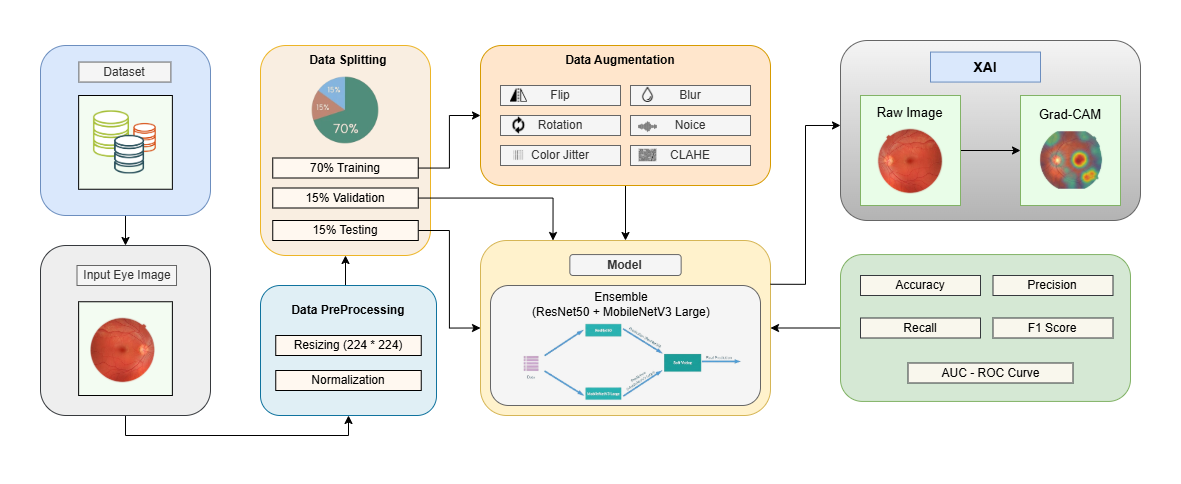
\includegraphics[width=0.9\textwidth]{Untitled Diagram.drawio.png}
    \caption{Complete system architecture of the proposed framework showing the end-to-end pipeline from data acquisition to explainable prediction.}
    \label{fig:architecture}
\end{figure*}

\subsection{Image Preprocessing Pipeline}

The resolution, colour balance and contrast of fundus images obtained from various clinical settings is variable because of the varying camera types, lighting conditions and imaging protocols. Our multi-stage preprocessing pipeline is an effective response to these challenges systematically. The images normally include a circle of retina surrounded by a large and uninformative black margin. All images are then resized to be the same size of $224 \times 224$ pixels to comply with the input size required by pre-trained models.

Raw pixel values (0-255) are first scaled to $[0, 1]$ by dividing by 255, then z-score normalized using ImageNet mean ($\mu = [0.485, 0.456, 0.406]$) and standard deviation ($\sigma = [0.229, 0.224, 0.225]$). Contrast Limited Adaptive Histogram Equalization(CLAHE) is used for blood vessels very much clear, done on small image tiles in parallel, clipping limit to not overemphasize noise. CLAHE improves the contrast of subtle structures, like microaneurysms, early cataract and fine vascular changes that may not be recognized due to uneven illumination \cite{paper2, paper15}.



\subsection{Data Augmentation Strategy}

To prevent overfitting on the small medical dataset, we only use extensive augmentation on the training set. Our augmentation strategy includes: (1) random horizontal and vertical flipping to simulate left/right eye captures; (2) random rotation up to $\pm$30\textdegree{} to handle camera positioning variations; (3) Applying color jitter to adjust brightness, contrast, saturation, and hue to simulate different camera models and lighting; (4) Gaussian blurring to simulate slightly out-of-focus captures; (5) Gaussian noise injection to force robust feature learning; and (6) random CLAHE application to train the model on both enhanced and unenhanced images.

\subsection{Deep Learning Architectures}

All models use ImageNet pre-trained weights with a custom classification head replacing the original 1,000-class output: Global Average Pooling $\rightarrow$ Dense(256, ReLU) $\rightarrow$ Dropout(0.5) $\rightarrow$ Dense(4, Sigmoid). The Sigmoid activation models each class independently, enabling multi-class output. Six widely used deep learning architectures are evaluated under identical experimental settings. ResNet50 (25.6M parameters) employs residual learning through skip connections to facilitate the training of deep networks while mitigating the vanishing gradient problem. VGG16 (138M parameters) is an example of the first generation of CNN architectures, made up of stacked $3\times3$ convolutional layers and max-pooling operators. DenseNet121 (8M parameters) is designed to enhance feature propagation in dense blocks by fully connecting all layers in the past, which allows for feature reusing with relatively small parameters. MobileNetV3-Large (4.2M parameters) is a lightweight architecture with depthwise separable convolution, inverted residual structure, and squeeze and excitation modules, which is used to extract features with computational efficiency. ConvNeXt-Tiny (27.8M parameters) introduces the new large $7\times7$ depthwise convolutions, GELU activation, and LayerNorm to the traditional CNN design. The Vision Transformer (ViT) (85.8M parameters) splits each input image into $16\times16$ patches and then applies multi-head self-attention-based Transformer encoder to model the long-range image interactions between the patches.


\subsection{Proposed Ensemble Model}

The custom ensemble is a combination of the two top performing architectures ResNet50 and MobileNetV3-Large, using soft voting (probability averaging), which is shown in Fig.~\ref{fig:ensemble_arch}.

{\textit{1) ResNet50 Branch:}} The first branch employs ResNet50 as the backbone network. The input image is processed through an initial convolutional layer followed by BatchNorm, ReLU activation, and MaxPool, before passing through four stages of residual blocks. A fully connected classification and Global Average Pooling layer produce the first probability vector, $P_{\text{ResNet}}$.

\textit{{2) MobileNetV3-Large Branch:}} The second branch employs MobileNetV3-Large as the backbone network. Feature extraction is performed using bottleneck structures with $1\times1$ convolutions for channel expansion, depthwise convolutions for spatial filtering, and Squeeze-and-Excitation modules that adaptively re-weight feature channels. The resulting feature representation is passed through the classification layer to produce the second probability vector, $P_{\text{Mobile}}$.

\textit{{3) Soft Voting Integration:}} The predicted probabilities from both branches are averaged element-wise as $P_{\text{final}} = \frac{1}{2}(P_{\text{ResNet}} + P_{\text{Mobile}})$, followed by thresholding at 0.5 to obtain the final multi-class prediction.


\begin{figure*}[!t]
    \centering
    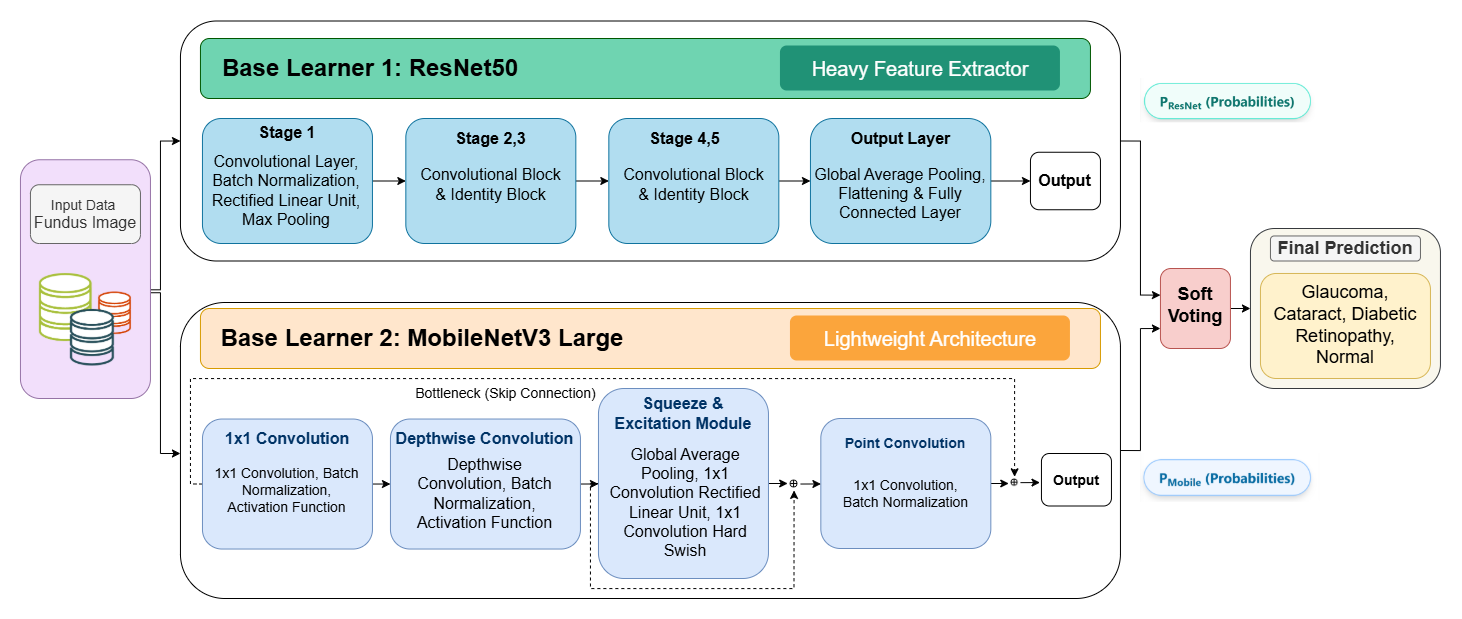
\includegraphics[width=0.9\textwidth]{Arc.drawio (1).png}
    \caption{Detailed architecture of the proposed ensemble model combining ResNet50 and MobileNetV3-Large via soft voting.}
    \label{fig:ensemble_arch}
\end{figure*}

\subsection{Training Configuration}

Table~\ref{tab:hyperparams} summarizes the hyperparameter settings used across all models. The Adam optimizer was chosen for its adaptive per-parameter learning rates. Binary Cross-Entropy loss treats each class independently, enabling multi-class training. ReduceLROnPlateau monitors validation loss and reduces the learning rate by a factor of 10 when improvement stalls for 3 consecutive epochs, allowing large initial steps with finer adjustments near convergence.

\begin{table}[!ht]
\centering
\caption{Hyperparameter configuration for model training.}
\label{tab:hyperparams}
\renewcommand{\arraystretch}{1.0}
\setlength{\tabcolsep}{4pt}
\begin{tabular}{ll}
\toprule
\textbf{Hyperparameter} & \textbf{Value} \\
\midrule
Optimizer & Adam \\
Initial learning rate & 0.0001 \\
Batch size & 32 \\
Number of epochs & 12 \\
Loss function & Binary Cross-Entropy \\
LR scheduler & ReduceLROnPlateau (factor=0.1, patience=3) \\
Early stopping patience & 5 epochs \\
Dropout rate & 0.5 \\
Input image size & $224 \times 224 \times 3$ \\
\bottomrule
\end{tabular}
\end{table}

\subsection{Grad-CAM for Clinical Interpretability}

Gradient-weighted Class Activation Mapping (Grad-CAM) generates visual heatmaps showing which image regions drive each prediction. For a target class $c$ the importance weight $\alpha_k^c$ of the $k$-th feature map $A^k$ of the final convolutional layer is calculated as follows:
\begin{equation}
\alpha_k^c = \frac{1}{Z} \sum_{i}\sum_{j} \frac{\partial y^c}{\partial A_{i,j}^k}
\end{equation}
where $Z$ is the number of spatial positions. The final heatmap is computed using a weighted combination and then ReLU to keep only the positive parts:
\begin{equation}
L^c_{\text{Grad-CAM}} = \text{ReLU}\left( \sum_{k} \alpha_k^c A^k \right),
\end{equation}
This produces a heat map, which, after being upsampled to match the dimensions of the input image, is then overlaid using a jet colormap (red = high importance, blue = low) and compared to the known pathological regions in order to verify that the attention of the model was the same as that of a clinician.

\section{Results and Discussion}

\subsection{Training Dynamics}

The training and validation loss over 12 epochs are shown in Fig.~\ref{fig:train_loss}. The training loss continues to decrease until epoch 12, with the value around 0.10, and the validation loss stabilizes around 0.15. Both curves are very similar throughout the epochs, showing very little overfitting and a good generalisation. The plot shows a smooth and monotonic decay without sharp peaks, which indicates a consistent optimization process and a suitable learning rate schedule.

\begin{figure}[!ht]
    \centering
    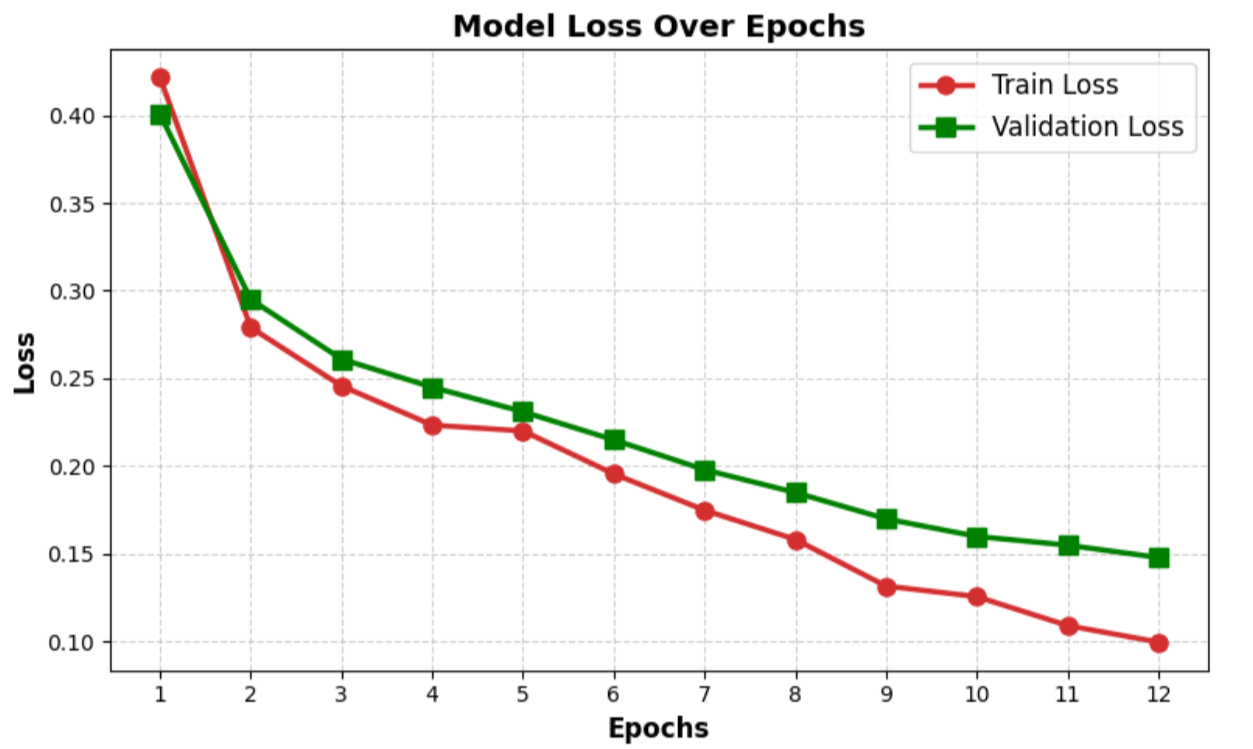
\includegraphics[width=0.78\columnwidth]{t vs v.png}
    \caption{Training and validation loss curves of the proposed ensemble model over 12 epochs.}
    \label{fig:train_loss}
\end{figure}

\subsection{Performance Benchmarking}

Table~\ref{tab:results} This is the full comparison between all seven models on the test set not used in the training. The Custom Ensemble has the best results on all of the four evaluation metrics.

\begin{table}[!ht]
    \centering
    \caption{Performance comparison of all benchmarked models on the held-out test set.}
    \label{tab:results}
    \resizebox{\columnwidth}{!}{%
    \begin{tabular}{@{}lcccc@{}}
        \toprule
        \textbf{Model} & \textbf{Accuracy} & \textbf{Precision} & \textbf{Recall} & \textbf{F1-Score} \\
        \midrule
        VGG16 & 91.48\% & 0.9237 & 0.9148 & 0.9139 \\
        Vision Transformer & 92.02\% & 0.9276 & 0.9202 & 0.9194 \\
        ConvNeXt-Tiny & 92.13\% & 0.9231 & 0.9213 & 0.9208 \\
        DenseNet121 & 92.35\% & 0.9275 & 0.9235 & 0.9232 \\
        ResNet50 & 92.79\% & 0.9330 & 0.9279 & 0.9275 \\
        MobileNetV3-Large & 93.22\% & 0.9368 & 0.9322 & 0.9318 \\
        \textbf{Custom Ensemble} & \textbf{93.77\%} & \textbf{0.9412} & \textbf{0.9377} & \textbf{0.9374} \\
        {\footnotesize \textbf{(ResNet50 + MobileNetV3-Large)}} & & & & \\
        \bottomrule
    \end{tabular}%
    }
\end{table}

The sequential design VGG16 (91.48\%) achieved the lowest, which is also supported by the lower F1-score (0.9139). ViT and ConvNeXt-Tiny achieved comparable results approximately 92\% accuracy, with ConvNeXt-Tiny being slightly better in terms of precision (0.9231 vs 0.9276), but this dataset size did not enable the self-attention mechanism of ViT to secure any significant advantage. Dense connectivity and compact design was a benefit for DenseNet121 (92.35\%). ResNet50 (92.79\%) had excellent performance by using residual learning. MobileNetV3-Large (93.22\%) achieved the highest balanced precision (0.9368) and F1 score (0.9318) among the individual models, indicating that NAS-optimized architectures could offer similar performance to heavier models, with implicit regularization. The Custom Ensemble (93.77\%) generated the best results through the combination of complementary strengths of ResNet50's deep residual features and MobileNetV3-Large's efficient attention-based features, reaching an impressive score of 0.9412 for precision.

\subsection{Confusion Matrix Analysis}

The confusion matrix (Fig.~\ref{fig:confusion}) shows detailed performance patterns of the ensemble model at the level of each class. Cataract had 0 misclassifications and 212/212 correct classifications; even though they are cloudy, they have a characteristic pattern that is easily visually distinguished from other conditions. Diabetic Retinopathy achieved an excellent performance (235/241 correct), especially due to the hemorrhages, exudates and microaneurysms that are characteristic of DR. Glaucoma did well (226/236 correct) but with some confusion. The weakest category was normal (169/226 correct) where 55 normal images were mis-classed as glaucoma.

This is a documented problem in automated systems and also for clinicians when diagnosing Normal-Glaucoma. Not all glaucoma patients will have an abnormal cup to disc ratio and some healthy patients will naturally have bigger optic cups that would appear like early glaucoma on 2D fundus images.

\begin{figure}[!ht]
    \centering
    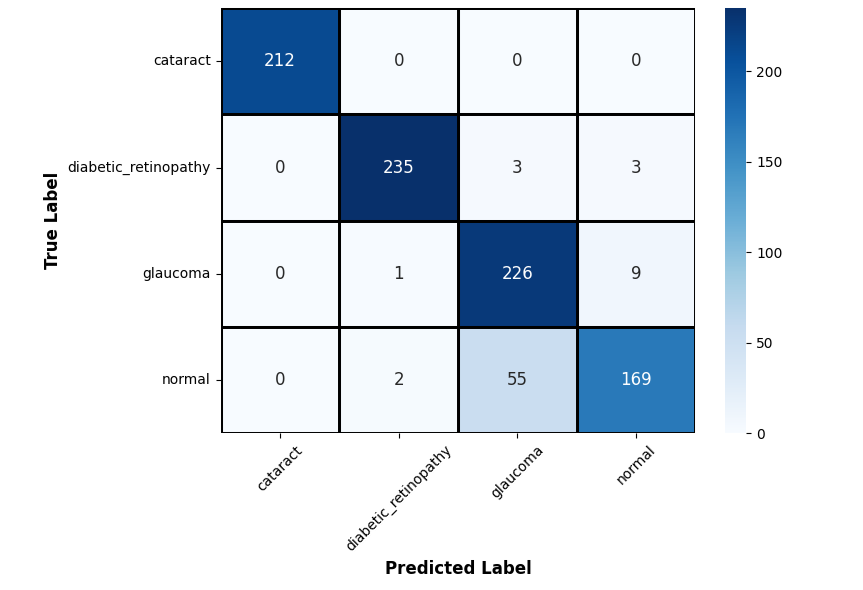
\includegraphics[width=\columnwidth]{Confusion Matrix.png}
    \caption{Confusion matrix of the ensemble model on the held-out test set showing per-class classification performance.}
    \label{fig:confusion}
\end{figure}

\subsection{ROC Curve and AUC Analysis}

The per-class ROC are shown in Fig.~\ref{fig:roc}. The AUC values are perfect, 1.000, for both DR and cataract, meaning that they are completely separable at all threshold values. Glaucoma (AUC = 0.983) and Normal (AUC = 0.981) have slightly lower, but still excellent, discrimination and corresponds to what is seen with the inter-class confusion. The values of these AUCs suggest a high level of reliability for initial clinical screening in our ensemble, especially for cataract and DR, where penalty for a misdiagnosis (false negative) might be circumvented by selecting suitable confidence thresholds.

\begin{figure}[!ht]
    \centering
    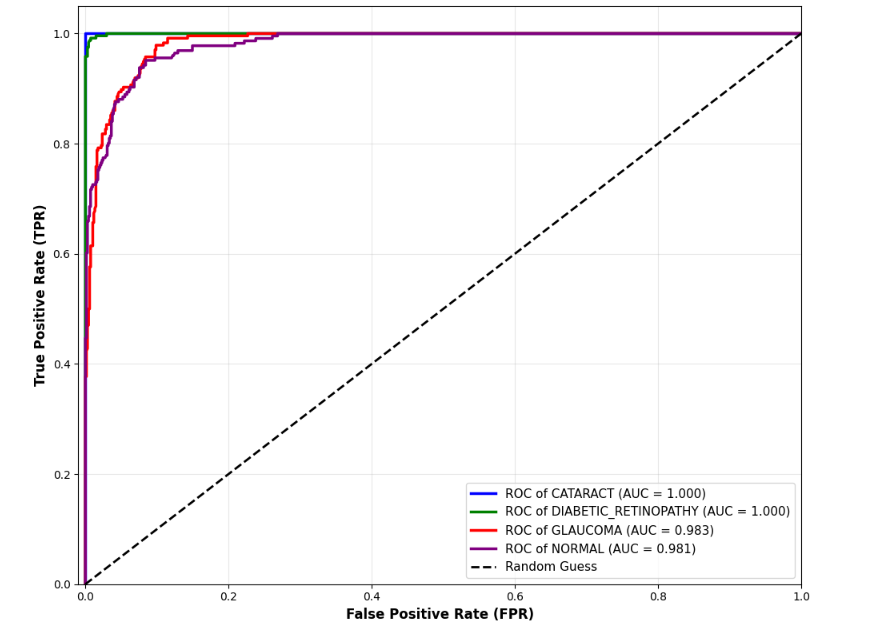
\includegraphics[width=\columnwidth]{ROC.png}
    \caption{Per-class ROC curves for the ensemble model with AUC scores.}
    \label{fig:roc}
\end{figure}

\subsection{Grad-CAM Interpretability Analysis}

Grad-CAM heat maps for some representative test images (figure~\ref{fig:gradcam}) show that the model focuses on clinically relevant areas. For Glaucoma, activation will focus on the optic disc, which corresponds to the clinical cup to disc ratio evaluation. For DR, the focus is spread throughout the macula and the peripheral retina, with areas of interest marking areas with exudates, microaneurysms and hemorrhages. In normal images, activation diminishes in a diffuse manner in the vascular arcades with no pathological focus. These patterns demonstrate that the model has learned features that are diagnostic and not just spurious correlations, which is why the model is used as a tool to clinically validate.

\begin{figure}[!ht]
    \centering
    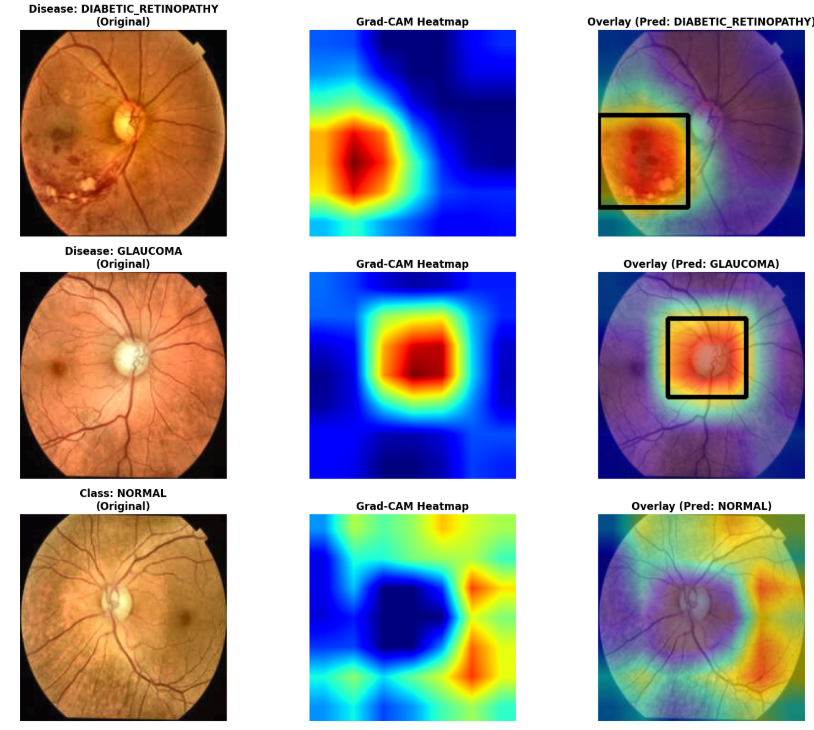
\includegraphics[width=\columnwidth]{gradCAM.png}
    \caption{Grad-CAM heatmaps for Glaucoma, Normal, and Diabetic Retinopathy classifications showing clinically meaningful attention regions.}
    \label{fig:gradcam}
\end{figure}

\subsection{Comparison with Other Existing Literature}

Table~\ref{tab:comparison} Conducts a comparison of our proposed framework with recent studies. Most of the current models are based on publicly available datasets (e.g. ODIR, Kaggle), but fail to provide explainability, whereas our model is based on a large unique clinical dataset from Sylhet Eye Hospital (6,086 images). While making direct comparisons of accuracy is always tricky because of different data sets and evaluation methods, our ResNet50-MobileNetV3 ensemble achieves the best in terms of accuracy (93.77\%) and F1-score (93.74\%). Moreover, it uniquely combines Grad-CAM for clinically reliable multi-class diagnosis in a transparent manner.
\begin{table}[!ht]
\centering
\caption{Comparison with recent studies.}
\label{tab:comparison}
\renewcommand{\arraystretch}{1.5}
\setlength{\tabcolsep}{4pt}
\resizebox{\columnwidth}{!}{%
\begin{tabular}{lllcccc}
\toprule
\textbf{Study} & \textbf{Dataset} & \textbf{\makecell[tl]{Model \\ + XAI}} & \textbf{Acc.(\%)} & \textbf{Pre.(\%)} & \textbf{Rec.(\%)} & \textbf{F1(\%)} \\
\midrule
Choo et al. \cite{paper17} & \makecell[tl]{Eye Disease Retinal \\ + Glaucoma Fundus \\ + ODIR + RFMiD} & \makecell[tl]{ResNet50 (TL) \\ + None} & 78.79 & 80.04 & 78.79 & 78.76 \\
Fahmy \cite{paper10} & Kaggle (4,217) & \makecell[tl]{Gabor + VGG-16 \\ + None} & 85.34 & -- & -- & -- \\
Chea \& Nam \cite{paper13} & \makecell[tl]{ORIGA \\ + IDRiD \\ + Messidor} & \makecell[tl]{ResNet \\ + None} & 85.79 & -- & 85.79 & -- \\
Mayowa-Majaro \cite{paper5} & Kaggle (4,217) & \makecell[tl]{DenseNet201 \\ + LIME} & 86.14 & 90.52 & 82.58 & -- \\
Khan et al. \cite{paper9} & ODIR-5K & \makecell[tl]{VGG-19 \\ + None} & 90.94 & 92.00 & 90.50 & 90.50 \\
Tuncer et al. \cite{paper12} & ODIR-5K & \makecell[tl]{HOG+LBP+XGBoost \\ + None} & 92.00 & 92.00 & 92.00 & 92.00 \\
\textbf{Ours} & \textbf{Sylhet (6,086)} & \textbf{\makecell[tl]{ResNet50+MobV3 Ens. \\ + Grad-CAM}} & \textbf{93.77} & \textbf{94.12} & \textbf{93.77} & \textbf{93.74} \\
\bottomrule
\end{tabular}%
}
\end{table}

\section{Conclusion and Future Work}

This research addressed the critical need for automated, reliable multi-class ocular disease screening by proposing an explainable deep learning framework for the classification of four major conditions (Cataract, Diabetic Retinopathy, Glaucoma, and Normal) from 2D fundus images. Through rigorous evaluation of seven diverse architectures, our Custom Ensemble consistently outperformed individual baselines. By combining ResNet50's deep residual features with MobileNetV3-Large's efficient attention mechanisms, the ensemble achieved a superior overall accuracy of 93.77\% and precision of 0.9412. 

Class-specific analysis revealed exceptional diagnostic capability, achieving perfect classification for Cataract and an AUC of 1.000 for both Cataract and Diabetic Retinopathy. Even with the challenge of physiological cupping overlap (55 false positives), the model continued to have a high AUC of 0.983. To guarantee clinical transparency, Grad-CAM was visually validated by the ensemble to correctly target medically relevant areas, including the optic disc for Glaucoma and retinal lesions for Diabetic Retinopathy. Future work aims to incorporate 3D OCT data to resolve this issue of the depth perception limitation of 2D fundus imaging and the confusion of Normal versus Glaucoma. We will also aim to include more diseases, federated learning and create a mobile screening app. In conclusion, this approach combines high diagnostic accuracy with clear explanations, marking a major advance in ensuring trustworthy AI-assisted screening in real-world clinical settings.
\enlargethispage{2\baselineskip}
\small
\begin{thebibliography}{00}
\setlength{\itemsep}{0pt}
\setlength{\parskip}{0pt}
\bibitem{paper1} M. N. Safwan, M. H. Mahadi, S. Rahman, S. I. Niha, and M. F. Mridha, ``KbFL-XAI: Explainable knowledge-based federated learning for eye disease diagnosis,'' \textit{Biomedical Engineering Advances}, Elsevier, 2024.
\bibitem{paper2} \c{S}. K{\i}l{\i}\c{c} and his colleagues published their paper entitled ``HybridVisionNet: An advanced hybrid deep learning framework for automated multi-class ocular disease diagnosis using fundus imaging,'' in the \textit{Ain Shams Engineering Journal} 2025, vol. 16, p. 103594.
\bibitem{paper3} E. S. Cutur and N. G. Inan, \textit{Multi-class classification of retinal eye diseases from ophthalmoscopy images using transfer learning-based vision transformers}, \textit{J. Imaging Informatics in Medicine} vol. 38, pp. 3110-3124, 2025.
\bibitem{paper4} J. Wang, L. Yang, Z. Huo, W. He, and J. Luo, ``Multi-label classification of fundus images with EfficientNet,'' \textit{IEEE Access}, vol. 8, pp. 212499-212508, 2020.
\bibitem{paper5} A. Mayowa-Majaro, ``Deep learning for eye disease detection with confidence estimation and explainable AI,'' \textit{IRE Journals}, vol. 7, no. 10, 2024.
\bibitem{paper6} A. Bhati, N. Gour, P. Khanna, and A. Ojha, ``Discriminative kernel convolution network for multi-label ophthalmic disease detection on imbalanced fundus image dataset,'' \textit{arXiv:2207.07918}, 2022.
\bibitem{paper7} E. H. Rachmawanto, ``Eye disease classification using deep learning convolutional neural networks,'' \textit{J. Soft Computing Exploration} 2024.
\bibitem{paper8} M. R. A. B. Soflaei and K. S. Zamini, ``Explainable deep learning for cataract detection in retinal images: A dual-eye and knowledge distillation approach,'' \textit{arXiv:2509.22696}, 2025.
\bibitem{paper9} M. S. Khan \textit{et al.}, ``Deep learning for ocular disease recognition: An inner-class balance,'' \textit{Computational Intelligence and Neuroscience}, Hindawi, 2022.
\bibitem{paper10} A. M. Fahmy, ``Eye diseases prediction and classification using deep learning techniques,'' \textit{Annals of Biostatistics and Biometric Applications}, vol. 6, no. 1, 2024.
\bibitem{paper12} H. I. Tuncer and D. Alt{\i}nel, Classification of eye diseases using machine learning with preprocessing, in \textit{Proc. 8th Int. IDAP Symp.}, IEEE, 2024, pp. 1-6.
\bibitem{paper13} N. Chea, Y. Nam, ``Classification of fundus images based on deep learning for detecting eye diseases,'' \textit{Computers, Materials and Continua}, 2021, Tech Science Press.
\bibitem{paper14} C. Chen, Q. Shao, K. Svistunova, and S. Ablameyko, ``Integrating deep learning eye disease classification with traditional Chinese medicine's five-round theory,'' \textit{SSRN preprint}, 2024.
\bibitem{paper15} O. Rayhan, A. A. Lamia, and S. Sharif, ``Improved ResNet18: An interpretable deep learning framework for automated eye-disease classification,'' in \textit{Proc.} IEEE MPCON}, 2026, pp. 443-448.
\bibitem{paper16} M. Jaradat, A. E. Yildirim, T. Babaqi, S. H. Al-Nimer, and D. Won, ``Eye disease classification using deep learning techniques,'' in \textit{Proc. IISE Annual Conf.}, 2023.
\bibitem{paper17} A. M. S. Choo \textit{et al.}, ``Multiclass eye disease classification using transfer learning approach,'' \textit{Int. J. Computing and Technology Education}, vol. 17, no. 4, 2025.
\bibitem{paper18} S. Dardouri and R. Alsohemi, ``Fundus image-based eye disease detection using EfficientNetB3 architecture,'' \textit{J. Imaging}, vol. 11, no. 8, p. 279, 2025.
\bibitem{paper24} P. K. Mannepalli, V. D. S. Baghela, A. Agrawal, P. Johri, S. S. Dubey and K. Parmar, ``Transfer learning for automated classification of eye disease in fundus images from a pretrained model,'' Traitement du Signal, vol. 41, no. 5, p. 20, 2024.
\bibitem{gradcam} R. R. Selvaraju, M. Cogswell, A. Das, R. Vedantam, D. Parikh, and D. Batra, ``Grad-CAM: Visual explanations from deep networks via gradient-based localization,'' in \textit{Proc. IEEE ICCV}, 2017, pp. 618-626.
\bibitem{dataset} Sylhet Eye Hospital and Laser Centre, ``Eye disease Classification Fundus image dataset,'' Kaggle. [Online]. Available: \url{https://www.kaggle.com/datasets/mahin661/eye-disease-classification-fundus-image-dataset}
\end{thebibliography}

\end{document}
